\chapter{Random Effects in a Naive Bayes Classifier}
\section{Introduction}
\subsection{Bootstrapping}
Bootstrapping was introduced in 1979 by Bradley Efron and triggered a major event in Statistics. At that time, researchers used to implement complicated and often inaccurate approximations to biases, variances, and other measures of uncertainity by computer simulations. In \cite{BootstrapMethods97}, Davison and Hinkley describe how resampling from the original data can be used to obtain reliable standard errors, confidence intervals, and other measures of uncertainity. Although literally sampling from the data initially was accepted as a fraud (new samples are selected with replacement from the original observation, with the result that some of the original observations are repeated more than once in the bootstrap sample), it turned out that a wide range of statistical problems could be tackled this way. As a result, the need to over-simplify complex problems got solved, and allowed quick approximate solutions. Another interesting feature of bootstrapping is that the variance is reduced, and therefore helps avoiding overfitting. Finally, bootstrapping over cross-validation allows to provide confidence intervals for the estimated value. For this reason, bootstrapping techniques are widely implemented in the field of machine learning (eg bagging). Especially in the situation of small and imbalanced datasets, bootstrapping seems a very interesting approach: since it is nearly impossible to obtain more \textit{true} minority samples, and since it is very hard to model the minority distribution in order to generate artificial samples along the original distribution (eg using Gibbs Sampling), selective sampling with replacement might prove an excellent solution to oversample the minority class. 

\newpage 
\subsection{Random Forests}\label{randomforest}
Random forests were introduced by Leo Breiman in 2001~\cite{Breiman01randomforests} and are a combination of tree predictors such that each tree depends on the values of a random vector sampled independently and with the same distribution for all trees in the forest. Like earlier techniques such as bagging - where to grow each tree a random selection (without replacement) is made from the examples in the training set - and random split criterion~\cite{Dietterich00anexperimental} - where at each node the split is selected at random from among the K best splits - they increase the level of random effects steering the classification process.  Today, random forests are becoming increasingly popular in many scientific fields such as genetics and bioinformatics, where random forests are used to assess the importance of predictor variables in high dimensional settings. As Strobl and Zeileis state~\cite{strobl08why}, their advantages are that they can cope with "small \textit{n} large \textit{p}" problems, complex interactions and even highly correlated predictor variables. Moreover, random forests allow accurate classification, and the generalization error converges a.s. to a limit as the number of trees in the forest becomes large.
\vspace{1cm}\\
\includegraphics[scale=0.8]{img/random_forest_thumb.png}


\newpage
\subsection{Random Naive Bayes}\label{rnb}
Since the invention of random forests, many studies have applied the technique in order to overcome complex problems regarding classification or regression. Although the original idea was applied to classification trees, Prinzie and Van Den Poel introduce Random Naive Bayes (RNB) as a new bagged classifier combining a forest of Naive Bayes classifiers estimated with randomly selected features~\cite{rmc07}. Hence, RNB is a bagged classifier
combining a ‘forest’ of \textit{B} NBs. Each \textit{b}th NB is estimated on a bootstrap sample \(S_b\) with \textit{m} randomly selected features.  As each \textit{b}th NB delivers continuous posterior probabilities, predictions in the ensemble are calculated by adjusted Majority Vote (aMV). Results showed that RNB outperform state-of-the art SVMs, together with a various set of other classifiers where random effects were introduced. Hence, the importance of random effects seems evident, and allows to improve many classification tasks such as noise robustness and reduction of variance.
\vspace{1cm}\\
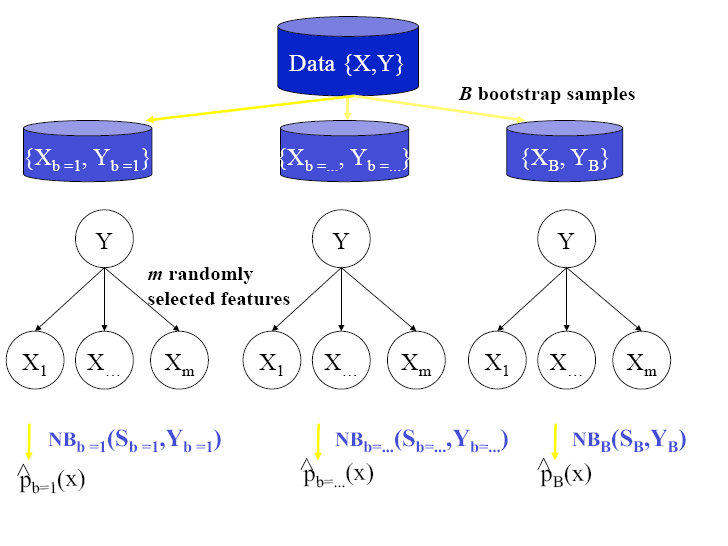
\includegraphics[scale=0.45]{img/rnb.png}


\newpage
\section{Random Naive Bayes with Feature-value Bootstrapping}
As a new approach to introduce random effects in Naive Bayes classifiers, we consider the sampling problem in imbalanced datasets. As discussed earlier, sampling proved an interesting solution to class imbalance, since it does not require alterations in the base classifiers and it moreover doesn't affect the interpretability of resulting models. However, it also has been discussed that simple oversample methods such as where the instances are basically copied or reweighted are not ideal and lead to overfitting. Although several samplers tackle this problem by creating synthetic samples based on the joint distribution (eg Gibbs Sampling) or their nearest neighbours (eg SMOTE), many of them pose no suitable solution to complex datasets where a select amount of instances are explained by a wide variety of features. The reason is simple: because of a lack of descriptive data (less than 30 positive training instances are present in this case) is combined with a large amount of interacting features, exhaustive techniques such as Gibbs Sampling is not only computiationally infeasible, but also impossible (since many of the dependencies are not covered in the dataset). In this section, we will introduce a new solution to class imbalances by exploiting Naive Bayes ' assumption of feature independence, the possibilities of bootstrapping and the predictive power of classifier ensembles.

\subsection{Approach}
In chapter~\ref{randomforest}, the technique of random forests was introduced as a technique which allows to cope with "small \textit{n} large \textit{p}" problems, complex interactions and even highly correlated predictor variables~\cite{strobl08why}. For this reason, they seem an excellent mean to solve the problem of imbalanced datasets, as advanced oversampling techniques are hindered by the lack of descriptive knowledge about the minority class. A first implementation of random forests in the  Naive Bayes classifier was introduced in 2007 by Prinzie and Van Den Poel~\cite{rmc07}, which was discussed in the previous chapter. Their implementation however is not focused on the problem of imbalanced datasets, and samples \textit{tree} populations by bootstrapping from the instance space, such as the original random forests do. When this technique would be applied to oversample a minority population,  sampled populations will only consist of duplicates and therefore bias the prior distributions of the independent features. For this reason, we introduce an extension to this approach in such way that bootstrapping is performed over the feature space (with the assumption of feature independence). This means that sampled (minority) populations will only consist of artificial instances, where the independent feature values are assigned by bootstrapping values from their original (minority) prior distributions. In order to keep computation complexity realistic, bootstrapping is not performed on the majority data, which is simply copied into each \textit{tree} population. This allows smaller forests to be built, as there will only exist a variability in the (oversampled) minority populations. For the same reason, all features are included in each separate sampled dataset, unlike RNB, where a random amount of features is selected.  

\newpage
The global approach of random naive bayes with feature-value bootstrapping (RNB-FvB) can be divided into three steps:

\begin{enumerate}
\item Create \textit{n} new (training) datasets by copying the majority data, and creating \(p\) minority examples by bootstrapping from the individual feature values in the original minority dataset. The parameter \(p\) is defined by forehand and describes the oversample ratio.
\item Train a Naive Bayes classifier on each separate dataset. Each trained classifier represents a tree in the random forest, which simply considers the aggregate of these \(n\) trained Naive Bayes classifiers.
\item Test data is predicted by averaging the votes of the individual trees (trained Naive Bayes classifiers) in the random forest.
\end{enumerate}
It should be clear that bootstrapping over the (individual) feature space is only valid when applied with a Naive Bayes classifier, as other classifiers will lose the power to catch the most important/informative feature interactions. This is exactly the reason why feature-value bootstrapping exploits the assumptions of a Naive Bayes classifier, and poses a valid solution to sampling in this context.
\vspace{1cm}\\
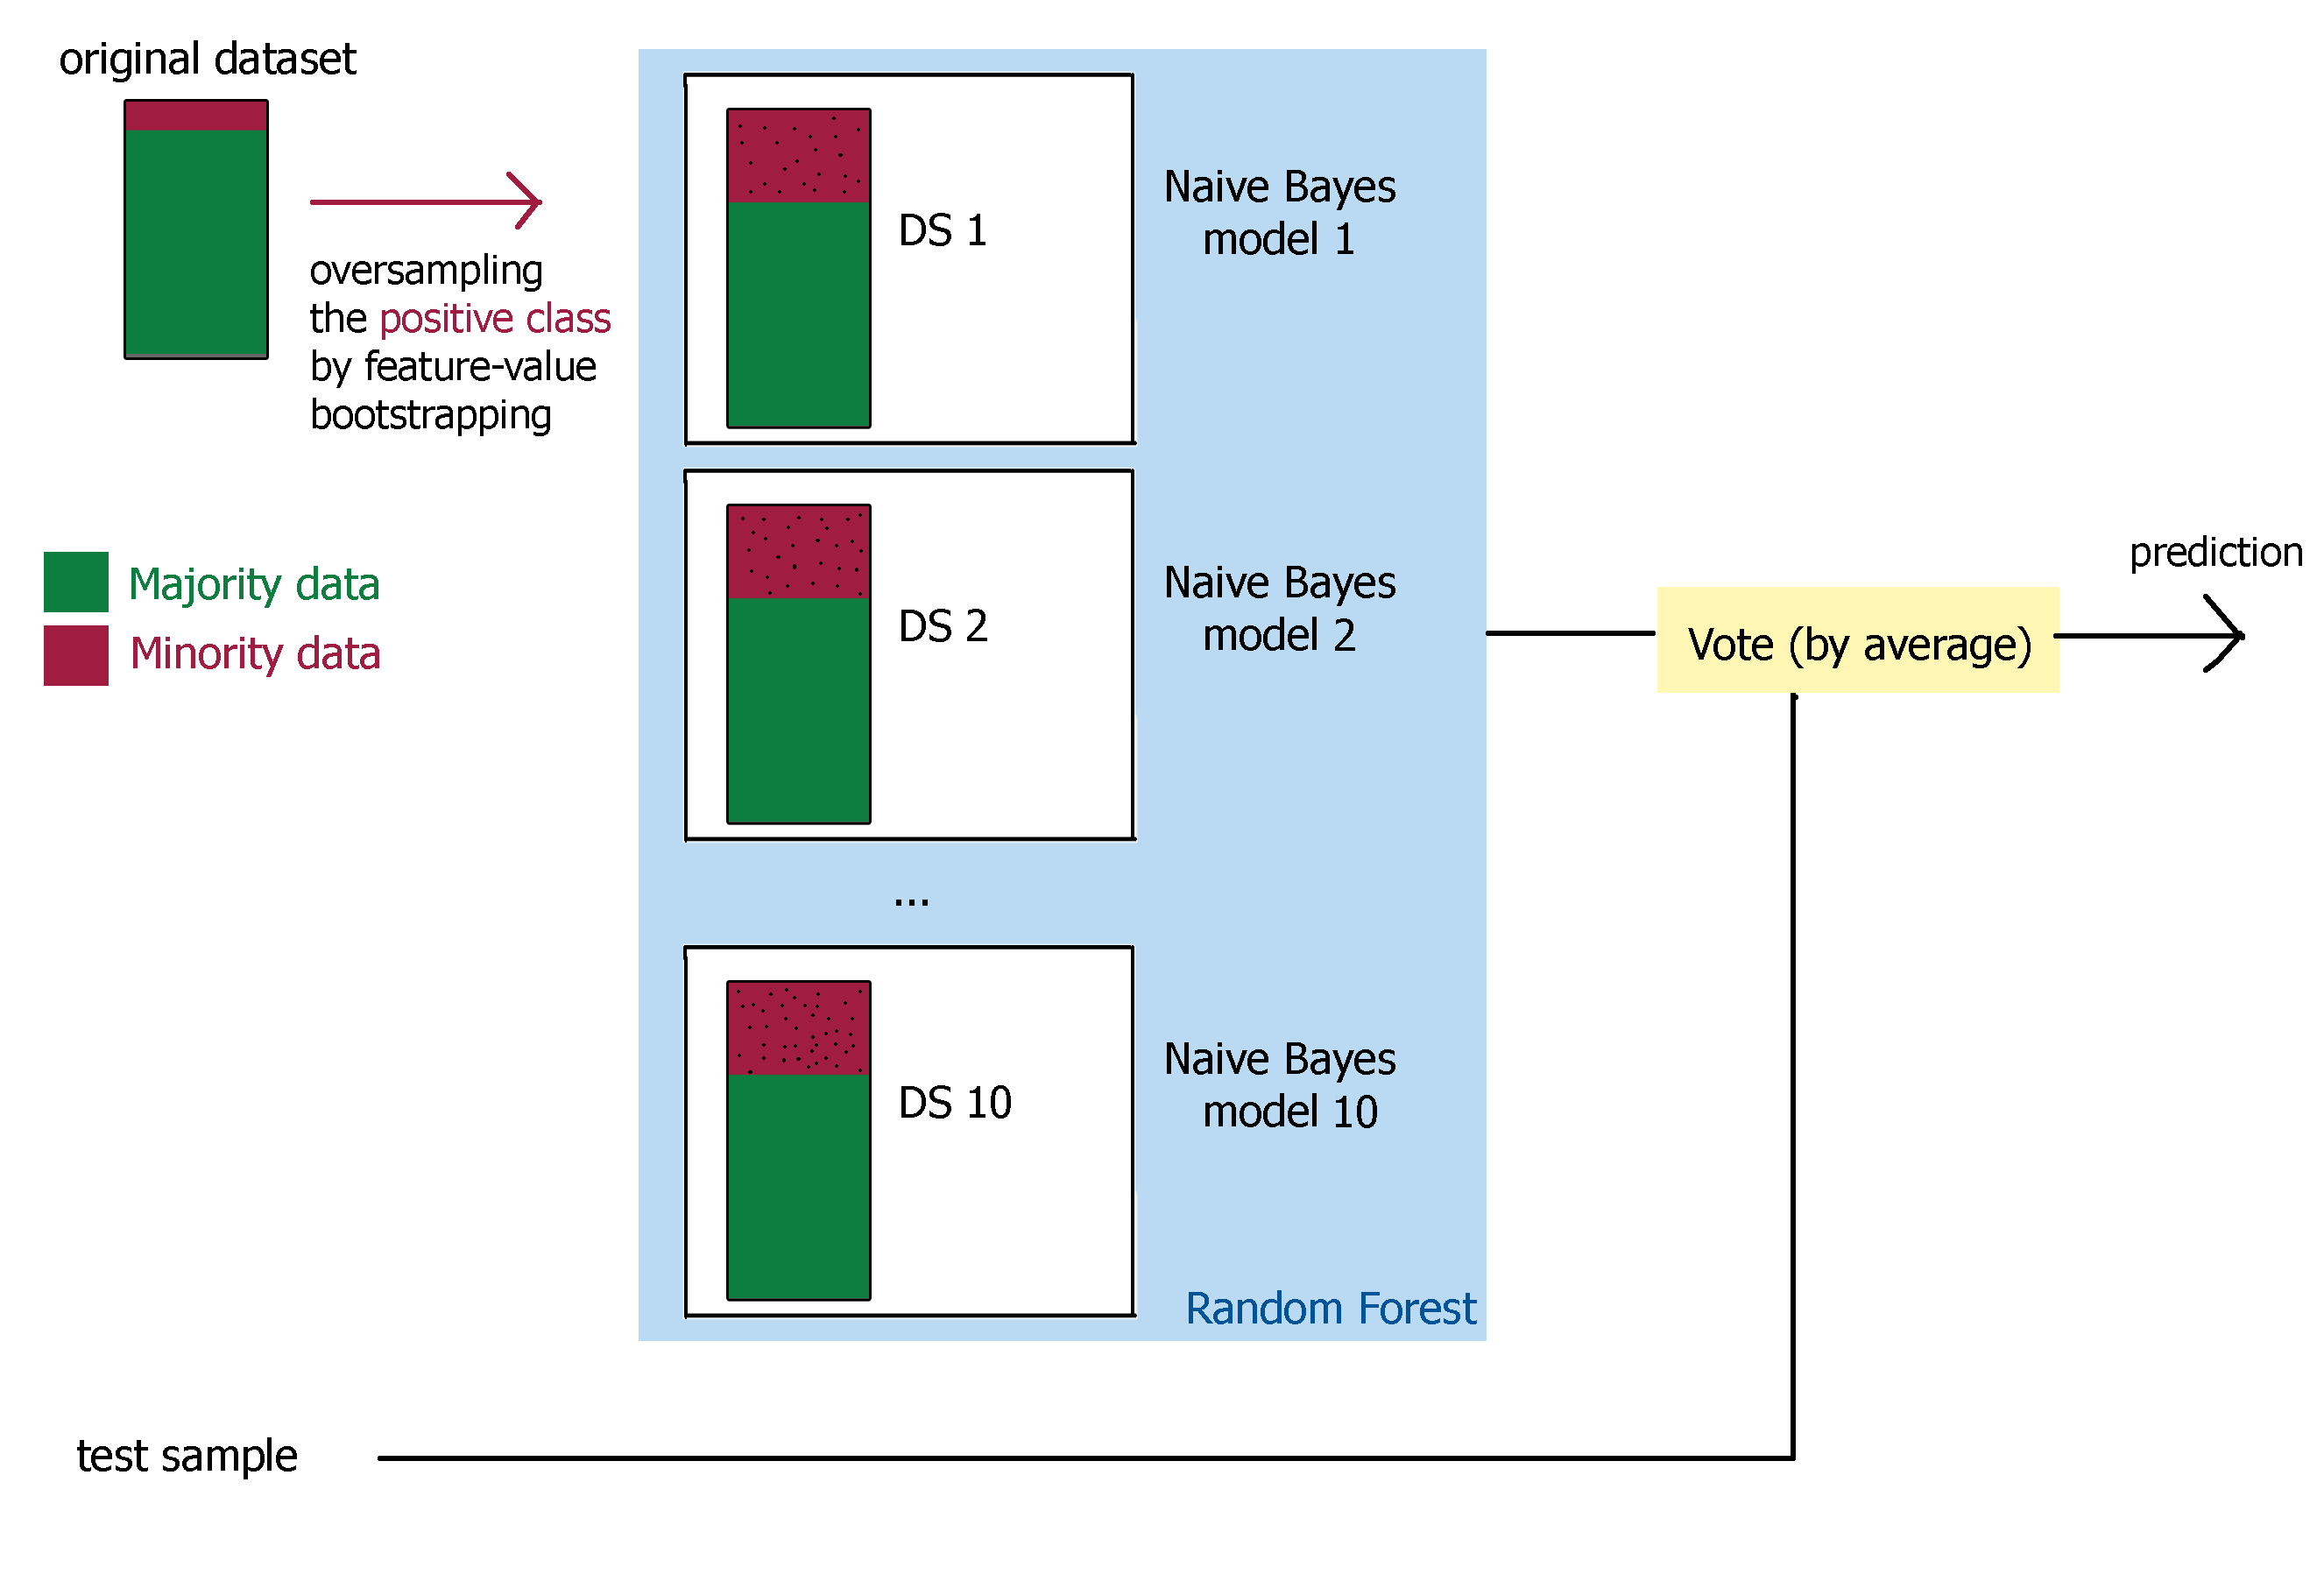
\includegraphics[scale=0.65]{img/rf.png}

\newpage
\subsubsection{Nominal Features}
In the case of nominal features, synthetic instances are given a value by simply bootstrapping from its prior distribution. For example, assume a feature F in the \textit{ill} class, which can take three values \textit{yes} (with \(P(F=yes|ill)=0.08\)), \textit{no} (with \(P(F=no|ill)=0.90\)) and \textit{don't know} (with \(P(F=dont know|ill)=0.02\)), with \(P_{missing}=0.03\) (meaning a value for feature F is missing in 3\% of all the instances). When a synthetic instance is created, a value for this feature (8\% for \textit{yes} and 90\% for \textit{no} and 2\% for \textit{don't know}) will be assigned by a probability of 97\% (and in 3\% of the cases be assigned as \textit{missing value}). 

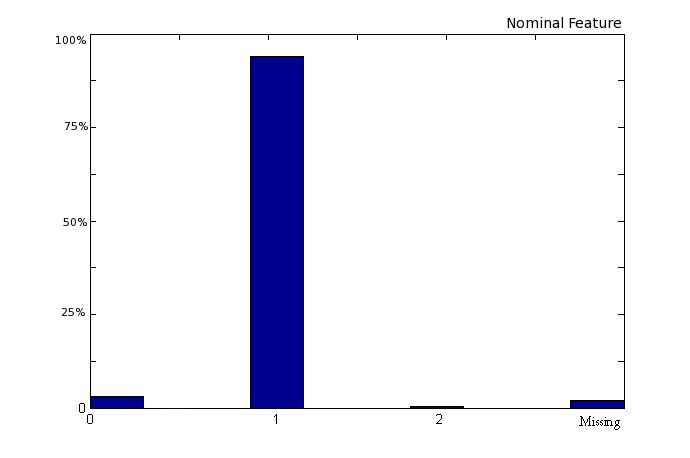
\includegraphics[scale=0.65]{img/nominalEst.png}



\newpage
\subsubsection{Numeric Features}
In the case of numeric features, a slightly more advanced technique is used to bootstrap the feature values. First, mean and variance of the prior distribution are estimated using Maximum Likelihood Estimation. These parameters are then used to generate new feature values along the prior (Gaussian) distribution. In order to overcome the generation of invalid values (eg the fitted Gaussian of a feature such as \textit{age} might also cover negative ages), valid value boundaries are defined (such as \(age \geq 0\)). When an invalid feature value is selected, a new value for the feature is calculated along the random distribution of \(N(0,max)\) where \textit{max} stands for the maximum value in the estimated gaussian. For example, assume \textit{age} is estimated by a Gaussian which captures the feature by a mean of 5, min of -2 and max of 12. It can then occur that a new instance will get a value of -1 for \textit{age}. In such case, \textit{age} will get a new value according to \(N(0,12)\). This actually means the original Gaussian distribution is augmented by a same amount over the value distribution which would have captured invalid values. Although it is clear that this approach is not a mathematical optimal solution, it tries in a simple way to add more variability into numerical features.\\\\

\includegraphics[scale=0.65]{img/gaussianEst.png}

\begin{landscape}
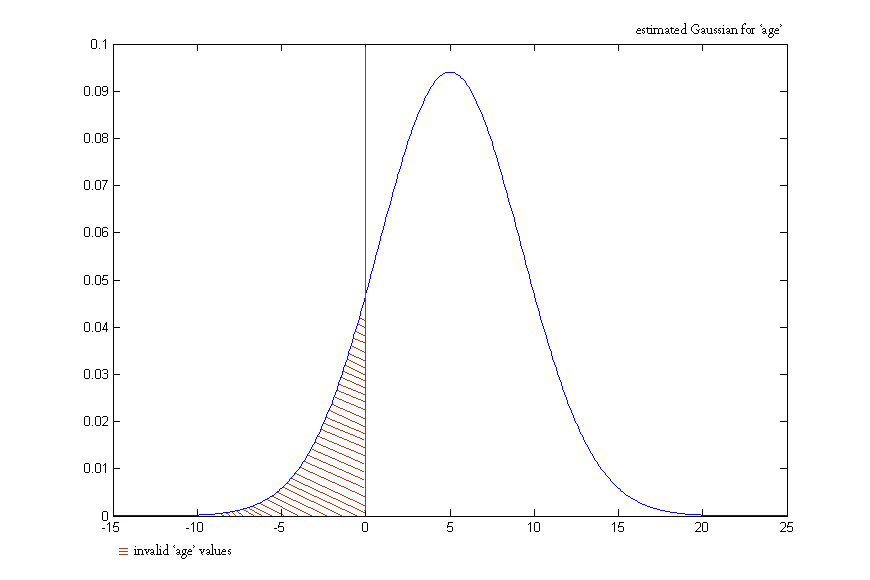
\includegraphics[scale=0.55]{img/AgeRegress.png} 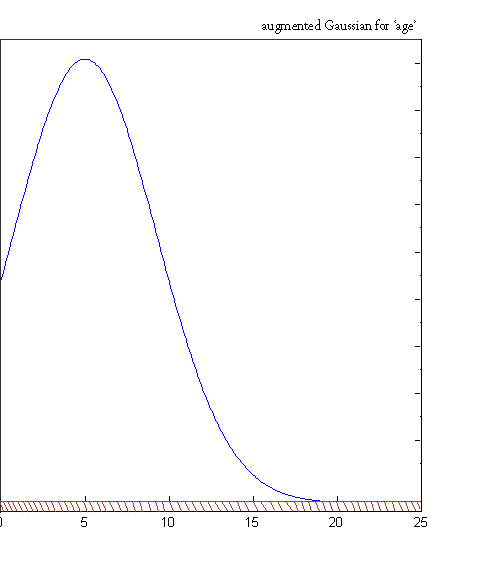
\includegraphics[scale=0.55]{img/AgeRegress2.png} 
\end{landscape}





